\PassOptionsToPackage{table}{xcolor}
\documentclass[aspectratio=169]{beamer}\usepackage[utf8]{inputenc}
\usepackage{lmodern}
\usepackage[english]{babel}
\usepackage{color}
\usepackage{amsmath,mathtools}
\usepackage{booktabs}
\usepackage{mathptmx}
\usepackage[11pt]{moresize}
\usepackage{hyperref}
\usepackage{commath}
\usepackage{bm}
\usepackage{subfigure}
\usepackage{siunitx}

\setbeamertemplate{navigation symbols}{}
\setbeamersize{text margin left=5mm,text margin right=5mm}
\setbeamertemplate{caption}[numbered]
\addtobeamertemplate{navigation symbols}{}{
\usebeamerfont{footline}
\usebeamercolor[fg]{footline}
\hspace{1em}
\insertframenumber/\inserttotalframenumber}

\newcommand{\R}{\mathbb{R}}
\newcommand{\E}{\mathbb{E}}
\newcommand{\N}{\mathbb{N}}
\newcommand{\Z}{\mathbb{Z}}
\newcommand{\V}{\mathbb{V}}
\newcommand{\Q}{\mathbb{Q}}
\newcommand{\K}{\mathbb{K}}
\newcommand{\C}{\mathbb{C}}
\newcommand{\T}{\mathbb{T}}
\newcommand{\I}{\mathbb{I}}
\DeclareMathOperator{\sign}{sign}

\title{Lamperti Transform for the processes X and V}
\subtitle{Renzo Miguel Caballero Rosas}

\begin{document}

\begin{frame}
\titlepage
\end{frame}

\setbeamercolor{background canvas}{bg=white!10}
\begin{frame}\frametitle{SDE for $X_t$:}

$\dif X_t=\left(\dot p_t-\theta_t(X_t-p_t)\right)\dif t+\sqrt{2\theta_t\alpha X_t(1-X_t)}\dif W_t\implies$
\begin{equation*}
\psi(X_t,t)=\int\frac{1}{\sqrt{2\theta_t\alpha u(1-u)}}\dif u\Bigg|_{u=X_t}=-\sqrt{\frac{2}{\alpha\theta_t}}\arcsin\left(\sqrt{1-X_t}\right).
\end{equation*}

\end{frame}


\setbeamercolor{background canvas}{bg=white!10}
\begin{frame}\frametitle{SDE for $V_t$:}

$\dif V_t=\underbrace{-\theta_tV_t}_{f(V_t,t)}\dif t+\underbrace{\sqrt{2\theta_t\alpha(V_t+p_t)(1-V_t-p_t)}}_{\sigma(V_t,t)}\dif W_t\implies$
\begin{equation*}
\psi(V_t,t)=\int\frac{1}{\sqrt{2\theta_t\alpha(u+p_t)(1-u-p_t)}}\dif u\Bigg|_{u=V_t}=-\sqrt{\frac{2}{\alpha\theta_t}}\arcsin\left(\sqrt{1-V_t-p_t}\right).
\end{equation*}
We can see that for every $t=t^*$, the primitive function of $\frac{1}{\sigma(v,t^*)}$ is well defined for all $v\in\left[-p(t^*),1-p(t^*)\right]\subset[-1,1]$ (recall $V_t=X_t-p_t$, and $x\in[0,1]$).

\end{frame}


\setbeamercolor{background canvas}{bg=white!10}
\begin{frame}\frametitle{SDE for $V_t$:}

We define $\Psi(V_t,t)=\int_{\epsilon}^u\frac{1}{\sigma(u,t)}\dif u\Big|_{u=V_t}$ where $\epsilon$ is in the space of $V_t$ (which depends on $p_t$).\\
\quad\\
We have that $V_t=X_t-p_t\iff V_t+p_t=X_t\implies0\leq V_t+p_t\leq1\iff-p_t\leq V_t\leq1-p_t$. Then, for each $t=t^*$, the space of the process is $[-p_{t^*},1-p_{t^*}]$. Now, notice that for all $p_{t^*}\in[0,1]$, we have that $q\in[-p_{t^*},1-p_{t^*}]$ if and only if $q=0$.\\
\quad\\
We conclude that if we want a fix value for $\epsilon$, necessarily we need to choose $\epsilon=0$.\\
\quad\\
We have that $\psi_v(V_t,t)=\Psi_v(V_t,t)$. However, $\psi_t(V_t,t)=\Psi_t(V_t,t)$ is in general no true, and $\Psi_t(V_t,t)$ has a more complicate expression.\\
\quad\\
If we choose $\epsilon=0$, we have that $\Psi_t(V_t,t)=\psi_t(V_t,t)+\frac{\dif}{\dif t}\int\frac{\dif u}{\sigma(u,t)}\Big|_{u=\epsilon=0}$.

\end{frame}


\setbeamercolor{background canvas}{bg=white!10}
\begin{frame}\frametitle{SDE for $V_t$:}

\begin{itemize}
\item $\Psi(V_t,t)=\psi(V_t,t)-\psi(\epsilon,t)\Big|_{\epsilon=0}=\sqrt{\frac{2}{\alpha\theta_t}}\left[\arcsin(\sqrt{1-\epsilon-p_t})-\arcsin(\sqrt{1-V_t-p_t})\right]\Big|_{\epsilon=0}=\sqrt{\frac{2}{\alpha\theta_t}}\left[\arcsin(\sqrt{1-p_t})-\arcsin(\sqrt{1-V_t-p_t})\right]$.
\item $\Psi_v(V_t,t)=\psi_v(V_t,t)=\frac{1}{\sigma(V_t,t)}$.
\item $\Psi_{vv}(V_t,t)=\psi_{vv}(V_t,t)=\frac{\dif}{\dif v}\left[\frac{1}{\sigma(V_t,t)}\right]=-\frac{\sigma_v(V_t,t)}{\sigma^2(V_t,t)}=-\frac{1}{\sigma^2(V_t,t)}\cdot\sqrt{\frac{\alpha\theta_t}{2}}\frac{1-2V_t-2p_t}{\sqrt{(V_t+p_t)(1-V_t-p_t)}}$.
\item $\psi_t(V_t,t)=\frac{\dot{p}_t}{\sqrt{2\alpha\theta_t}(V_t+p_t)(1-V_t-p_t)}+\frac{\alpha\dot{\theta}_t\arcsin(\sqrt{1-V_t-p_t})}{\sqrt{2}(\alpha\theta_t)^{3/2}}$.
\item $\Psi_t(V_t,t)=\psi_t(V_t,t)-\psi_t(\epsilon,t)\Big|_{\epsilon=0}=\frac{\dot{p}_t}{\sqrt{2\alpha\theta_t(V_t+p_t)(1-V_t-p_t)}}+\frac{\alpha\dot{\theta}_t\arcsin(\sqrt{1-V_t-p_t})}{\sqrt{2}(\alpha\theta_t)^{3/2}}-\frac{\dot{p}_t}{\sqrt{2\alpha\theta_t(\alert{0}+p_t)(1\alert{-0}-p_t)}}-\frac{\alpha\dot{\theta}_t\arcsin(\sqrt{1\alert{-0}-p_t})}{\sqrt{2}(\alpha\theta_t)^{3/2}}=\frac{1}{\sqrt{2\alpha\theta_t}}\left(\frac{\dot{p}_t}{\sqrt{(V_t+p_t)(1-V_t-p_t)}}+\frac{\alpha\dot{\theta}_t\arcsin(\sqrt{1-V_t-p_t})}{\alpha\theta_t}-\frac{\dot{p}_t}{\sqrt{(\alert{0}+p_t)(1\alert{-0}-p_t)}}-\frac{\alpha\dot{\theta}_t\arcsin(\sqrt{1\alert{-0}-p_t})}{\alpha\theta_t}\right)$.
\end{itemize}

\end{frame}


\setbeamercolor{background canvas}{bg=white!20}
\begin{frame}\frametitle{SDE for $Z_t=\Psi(V_t,t)$: ({\color{green}Verified with Mathematica})}

By It\^o's lemma:
\begin{equation*}
\dif Z_t=\left({\color{blue}\Psi_t}+\Psi_v\cdot f+\alert{\frac{1}{2}\Psi_{vv}\cdot\sigma^2}\right)\dif t+\Psi_v\cdot\sigma\dif W_t.
\end{equation*}
If we substitute the terms related with $\Psi(V_t,t)$:
\begin{equation*}
{\footnotesize
\begin{split}
\dif Z_t=&\Bigg[{\color{blue}\frac{1}{\sqrt{2\alpha\theta_t}}\left(\frac{\dot{p}_t}{\sqrt{(V_t+p_t)(1-V_t-p_t)}}+\frac{\alpha\dot{\theta}_t\arcsin(\sqrt{1-V_t-p_t})}{\alpha\theta_t}-\frac{\dot{p}_t}{\sqrt{(p_t)(1-p_t)}}-\frac{\alpha\dot{\theta}_t\arcsin(\sqrt{1-p_t})}{\alpha\theta_t}\right)}\\
&-\frac{\theta_tV_t}{\sqrt{2\alpha\theta_t(V_t+p_t)(1-V_t-p_t)}}\alert{-\frac{1}{2}\sqrt{\frac{\alpha\theta_t}{2}}\frac{1-2V_t-2p_t}{\sqrt{(V_t+p_t)(1-V_t-p_t)}}}\Bigg]\dif t+1\cdot \dif W_t.
\end{split}}
\end{equation*}

\end{frame}


\setbeamercolor{background canvas}{bg=white!10}
\begin{frame}\frametitle{SDE for $Z_t=\psi(V_t,t)$: ({\color{green}Verified with Mathematica})}

By It\^o's lemma, if $\psi(v,t)$ is $C^2([-p_t,1-p_t])$ for $v$ and $C^1([0,T])$ for $t$, then:
\begin{equation*}
\dif Z_t=\left({\color{blue}\psi_t}+\psi_v\cdot f+\alert{\frac{1}{2}\psi_{vv}\cdot\sigma^2}\right)\dif t+\psi_v\cdot\sigma\dif W_t.
\end{equation*}
If we substitute the terms related with $\psi(V_t,t)$:
\begin{equation*}
{\footnotesize
\begin{split}
\dif Z_t=&\Bigg[{\color{blue}\frac{1}{\sqrt{2\alpha\theta_t}}\left(\frac{\dot{p}_t}{\sqrt{(V_t+p_t)(1-V_t-p_t)}}+\frac{\alpha\dot{\theta}_t\arcsin(\sqrt{1-V_t-p_t})}{\alpha\theta_t}\right)}\\
&-\frac{\theta_tV_t}{\sqrt{2\alpha\theta_t(V_t+p_t)(1-V_t-p_t)}}\alert{-\frac{1}{2}\sqrt{\frac{\alpha\theta_t}{2}}\frac{1-2V_t-2p_t}{\sqrt{(V_t+p_t)(1-V_t-p_t)}}}\Bigg]\dif t+1\cdot \dif W_t.
\end{split}}
\end{equation*}
{\footnotesize
Recall $\alert{Z_t=-\sqrt{\frac{2}{\alpha\theta_t}}\arcsin\left(\sqrt{1-V_t-p_t}\right)}$. Then, we have the next identities: \textbf{1)} $\sqrt{1-V_t-p_t}=\sin\left(-Z_t\sqrt{\frac{\alpha\theta_t}{2}}\right)$, \textbf{2)} $1-V_t-p_t=\sin^2\left(-Z_t\sqrt{\frac{\alpha\theta_t}{2}}\right)$, and \textbf{3)} $V_t+p_t=1-\sin^2\left(-Z_t\sqrt{\frac{\alpha\theta_t}{2}}\right)$.}
\end{frame}


\setbeamercolor{background canvas}{bg=white!10}
\begin{frame}\frametitle{SDE for $Z_t=\psi(V_t,t)$:}

\begin{equation*}
{\scriptsize
\begin{split}
\dif Z_t=&\left[{\color{blue}\frac{1}{\sqrt{2\alpha\theta_t}}\left(\frac{\dot{p}_t}{\sqrt{\left(1-\sin^2\left(-Z_t\sqrt{\frac{\alpha\theta_t}{2}}\right)\right)\left(\sin^2\left(-Z_t\sqrt{\frac{\alpha\theta_t}{2}}\right)\right)}}+\frac{\dot{\theta}_t\left(-Z_t\sqrt{\frac{\alpha\theta_t}{2}}\right)}{\theta_t}\right)}\right.\\
&-\frac{\theta_t\left(1-p_t-\sin^2\left(-Z_t\sqrt{\frac{\alpha\theta_t}{2}}\right)\right)}{\sqrt{2\alpha\theta_t\left(1-\sin^2\left(-Z_t\sqrt{\frac{\alpha\theta_t}{2}}\right)\right)\left(\sin^2\left(-Z_t\sqrt{\frac{\alpha\theta_t}{2}}\right)\right)}}\\
&\left.\alert{-\frac{1}{2}\sqrt{\frac{\alpha\theta_t}{2}}\frac{1-2\left(1-\sin^2\left(-Z_t\sqrt{\frac{\alpha\theta_t}{2}}\right)\right)}{\sqrt{\left(1-\sin^2\left(-Z_t\sqrt{\frac{\alpha\theta_t}{2}}\right)\right)\left(\sin^2\left(-Z_t\sqrt{\frac{\alpha\theta_t}{2}}\right)\right)}}}\right]\dif t+1\cdot \dif W_t.
\end{split}}
\end{equation*}

\end{frame}


\setbeamercolor{background canvas}{bg=white!10}
\begin{frame}\frametitle{Range for $Z_t=\psi(V_t,t)$:}

We have that $Z_t=-\sqrt{\frac{2}{\alpha\theta_t}}\arcsin\left(\sqrt{1-V_t-p_t}\right)=-\sqrt{\frac{2}{\alpha\theta_t}}\arcsin\left(\sqrt{1-X_t}\right)$, where $X_t\in[0,1]$ almost sure. Then, we have that $Z_t\in\left[-\sqrt{\frac{2}{\alpha\theta_t}}\frac{\pi}{2},0\right]=\left[-\frac{\pi}{\sqrt{2\alpha\theta_t}},0\right]$, because $\arcsin\left([0,1]\right)=\left[0,\frac{\pi}{2}\right]$.\\
\quad\\
\graphicspath{{../../Mathematica_Files/}}
\begin{figure}[ht!]
\centering
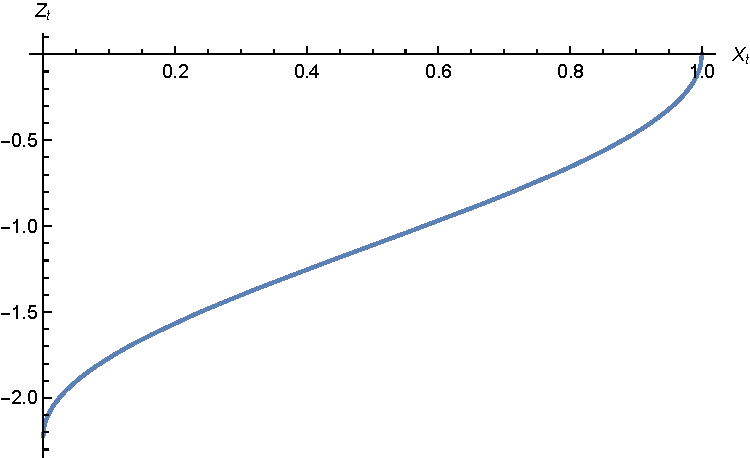
\includegraphics[width=0.3\textwidth]{Range_Z.pdf}
\caption{Plot of $Z_t$ as a function of $X_t$ from 0 to 1. We choose $\alpha=1/2$, and $\theta_t=1$. Notice that $Z_t(0)=-\frac{\pi}{\sqrt{2}}$, and $Z_t(1)=0$.}
\end{figure}

\end{frame}


\setbeamercolor{background canvas}{bg=white!10}
\begin{frame}\frametitle{SDE for $Z_t=\psi(V_t,t)$ with the c.o.v. $Y_t=Z_t\sqrt{\frac{\alpha\theta_t}{2}}$:}
We have that $Z_t\in\left[-\frac{\pi}{\sqrt{2\alpha\theta_t}},0\right]\iff Y_t\in\left[-\frac{\pi}{2},0\right]$.
\begin{equation*}
{\footnotesize
\begin{split}
\dif Z_t=&\left[{\color{blue}\frac{1}{\sqrt{2\alpha\theta_t}}\left(\frac{\dot{p}_t}{\sqrt{\left(1-\sin^2\left(Y_t\right)\right)\left(\sin^2\left(Y_t\right)\right)}}-\frac{\dot{\theta}_tY_t}{\theta_t}\right)}\right.\\
&-\frac{\theta_t\left(1-p_t-\sin^2\left(Y_t\right)\right)}{\sqrt{2\alpha\theta_t\left(1-\sin^2\left(Y_t\right)\right)\left(\sin^2\left(Y_t\right)\right)}}\\
&\left.\alert{-\frac{1}{2}\sqrt{\frac{\alpha\theta_t}{2}}\frac{1-2\left(1-\sin^2\left(Y_t\right)\right)}{\sqrt{\left(1-\sin^2\left(Y_t\right)\right)\left(\sin^2\left(Y_t\right)\right)}}}\right]\dif t+1\cdot \dif W_t.
\end{split}}
\end{equation*}

\end{frame}


\setbeamercolor{background canvas}{bg=red!30}
\begin{frame}\frametitle{SDE for $Z_t=\psi(V_t,t)$: Singularity in $Z_t=-\frac{\pi}{\sqrt{2\alpha\theta_t}}$, and $Z_t=0$}

We call $f_Z(Z_t,t)$ to the drift of $Z_t$. We define $Y_t=Z_t\sqrt{\frac{\alpha\theta_t}{2}}$, notice that $Y_t(Z_t=0)=0$, and $Y_t\left(Z_t=-\frac{\pi}{\sqrt{2\alpha\theta_t}}\right)=-\frac{\pi}{2}$. Now, we define $\hat{f}_Z$ a simplified version of $f_Z$ which has the same limits in the spatial boundaries.\\
We have that:
\begin{equation*}
\hat{f}_Z(y,t)={\color{blue}\left[\frac{\dot{p}_t}{\sqrt{2\alpha\theta_t}}\right]\frac{1}{(1-\sin^2(y))\sin^2(y)}}.
\end{equation*}
We have the next limits for some fixed $t$:
$$\lim_{y\to0^-}\hat{f}_Z(y,t)=\lim_{y\to-\frac{\pi}{2}^+}\hat{f}_Z(y,t)=\infty\times\sign(\dot{p}_t).$$

\alert{This result is a bit scaring because the sing depends on $\dot{p}_t$ when the process $Y_t$ touch the boundaries, not for the forecast $p_t$. LIMITS MAY BE WRONG! CHECK WELL!}

\end{frame}


\setbeamercolor{background canvas}{bg=white!10}
\begin{frame}\frametitle{What about the forecast $p(t)$?}

\begin{columns}[c]

\column{.6\textwidth}
We do not have control about the input $p(t)$. However, as it is discrete, we can choose how to make it continuous.\\
\quad\\
If we have a measurement every $\Delta t$-intervals, and we realize linear interpolation, then $|\dot{p}|\leq\frac{1}{\Delta t}$ as $p(t)\in[0,1]$. In our concrete case we have that $\frac{1}{\Delta t}=144$.\\
Theoretically, $\dot{p}(t)$ is not defined at the measurement times, and it is constant in the time between consecutive measurements.\\
\quad\\
In the case of $\ddot{p}(t)$, theoretically it is zero a.e., and it has Dirac's deltas at the measurement times.

\column{.3\textwidth}
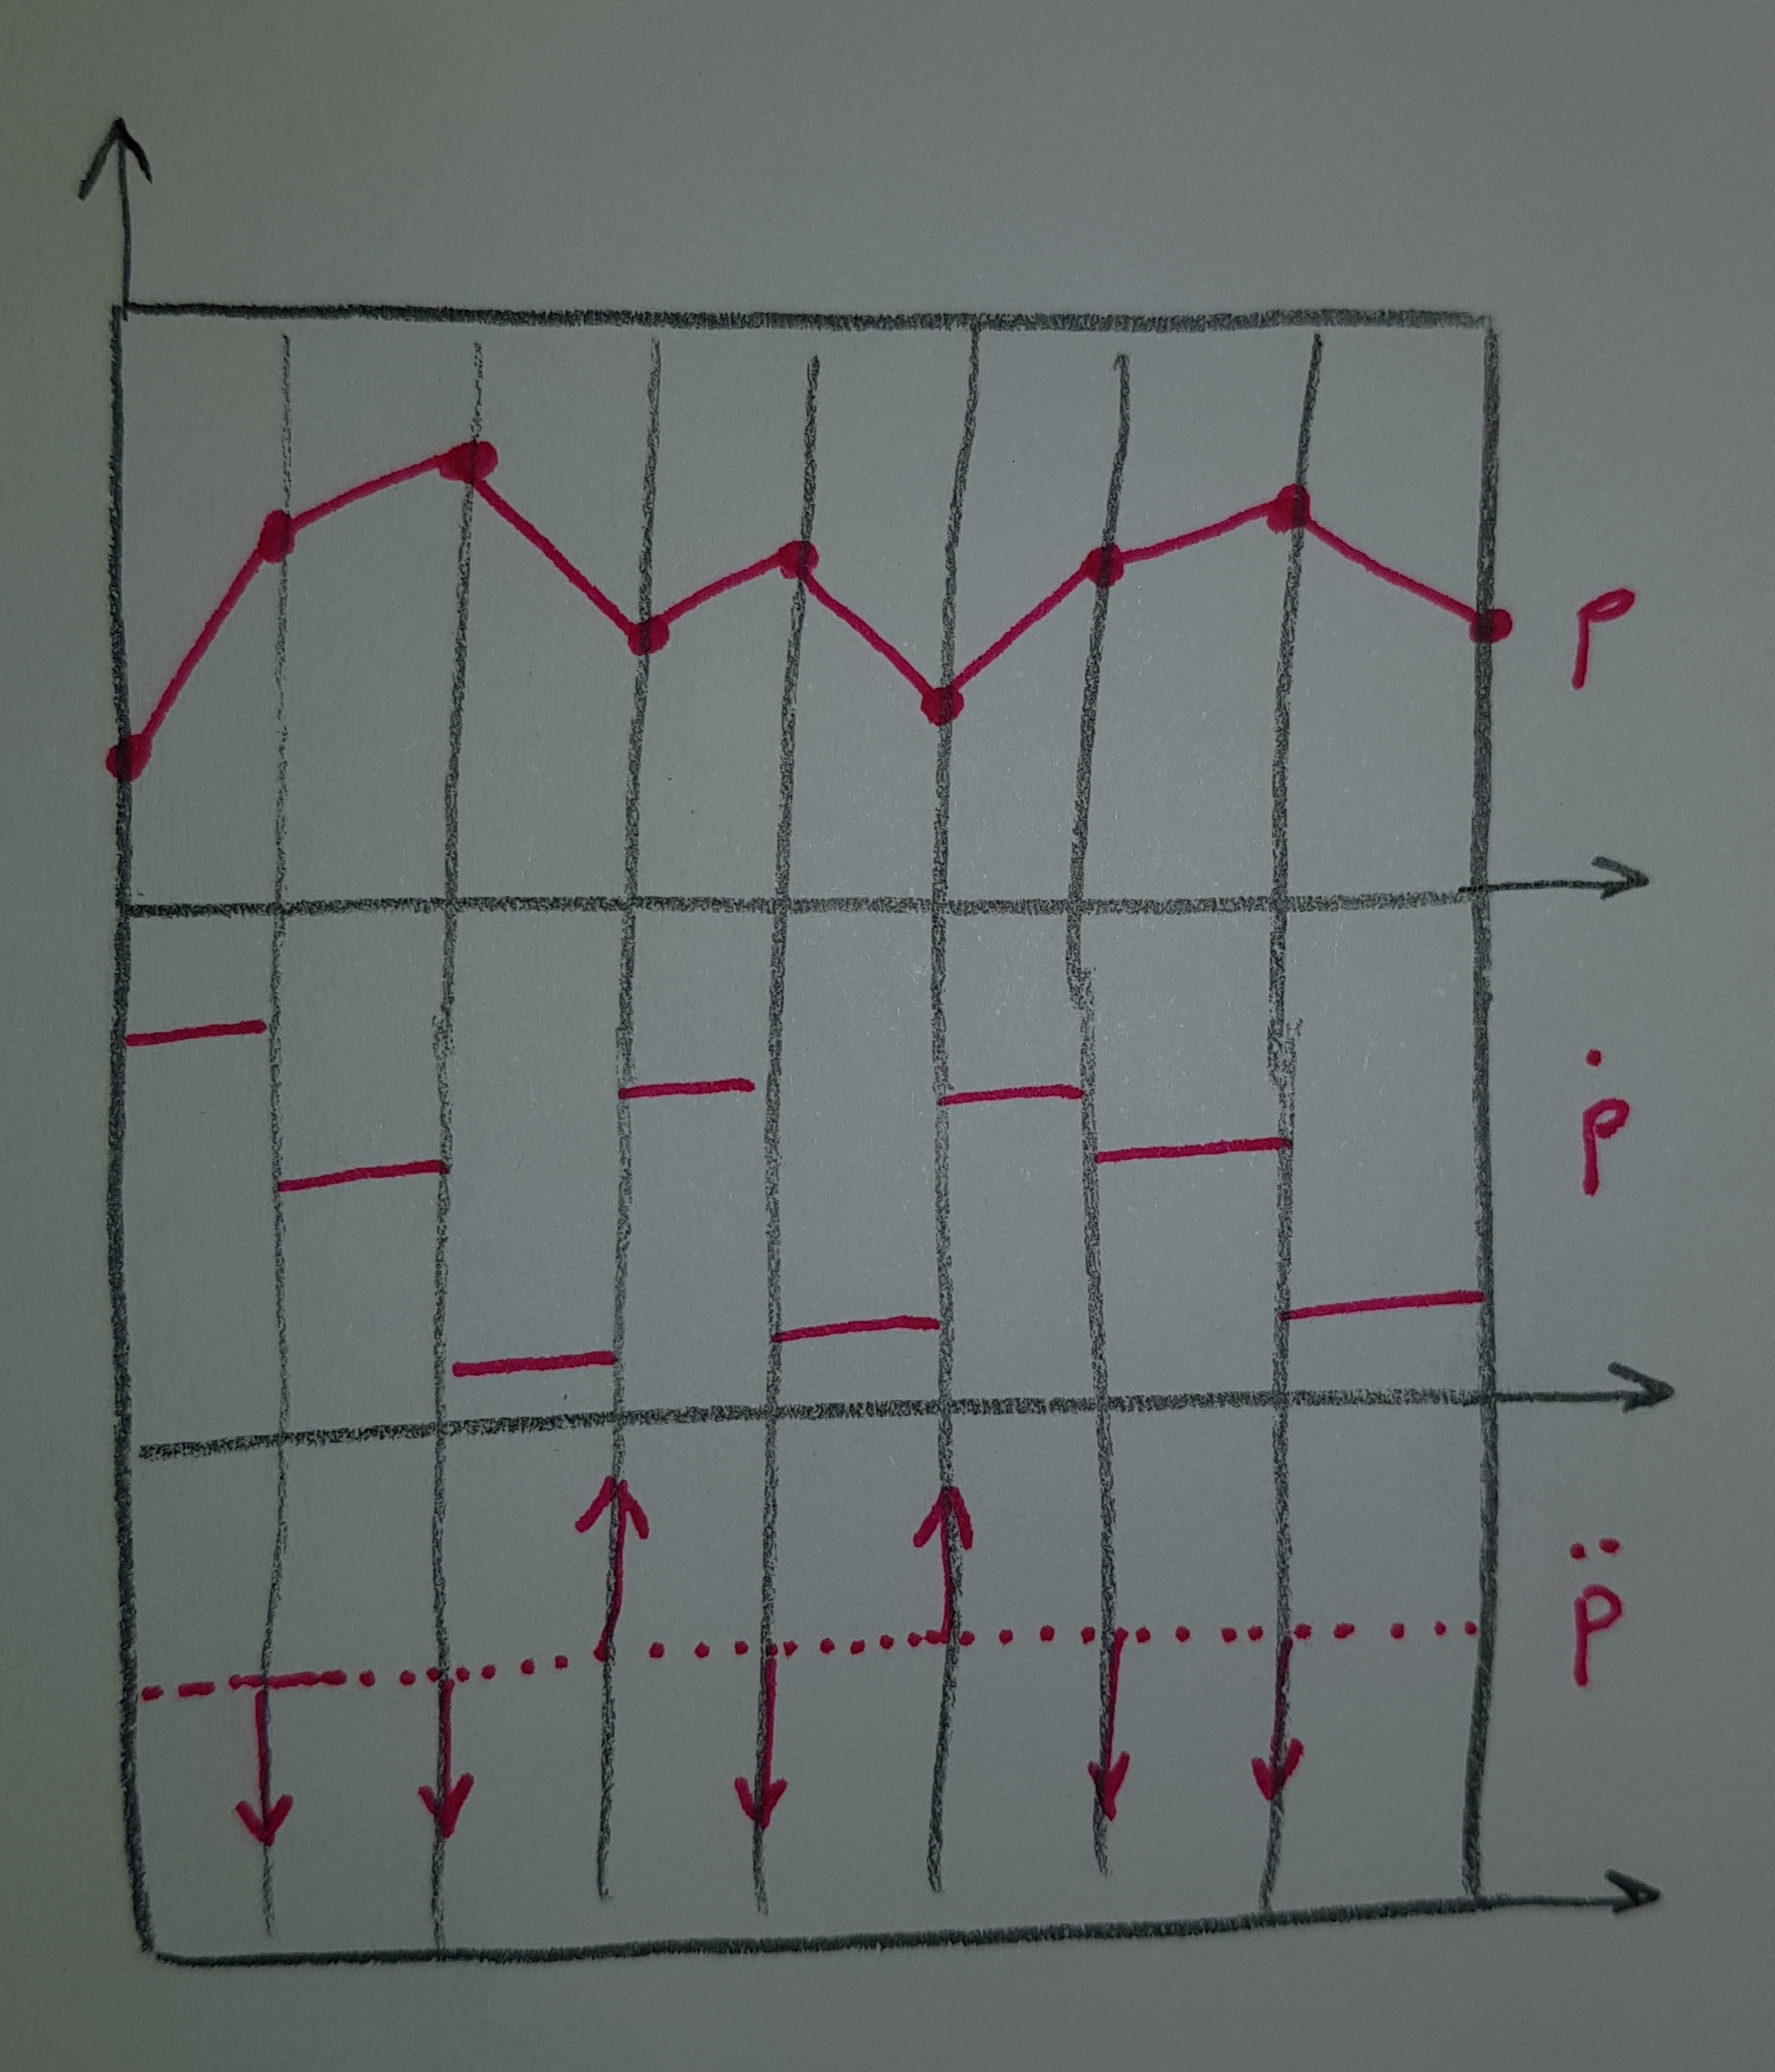
\includegraphics[width=0.9\columnwidth]{20200224_180726.jpg}

\end{columns}

\end{frame}


\setbeamercolor{background canvas}{bg=white!10}
\begin{frame}\frametitle{What about $\dot{\theta}_t$?}

\begin{equation*}
\dot{\theta}_t=\begin{cases}
\frac{\sign(\dot{p}_t)\ddot{p}_tp_t-|\dot{p}_t|\dot{p}_t}{p_t^2}\quad&\text{if}\quad|\dot{p}_t|>\theta_0p_t\ \text{\textbf{and}}\ p_t<\frac{1}{2}\\
\frac{\sign(\dot{p}_t)\ddot{p}_t(1-p_t)+|\dot{p}_t|\dot{p}_t}{(1-p_t)^2}\quad&\text{if}\quad|\dot{p}_t|>\theta_0(1-p_t)\ \text{\textbf{and}}\ p_t\geq\frac{1}{2}\\
0\quad&\text{otherwise}.
\end{cases}
\end{equation*}
\quad\\
\quad\\

\begin{columns}[c]

\column{.6\textwidth}
We need to take care of the extremes $p_t\approx0$ and $1-p_t\approx0$.\\
We will assume that always all the term involving $\ddot{p}_t$ is very small.

\column{.3\textwidth}
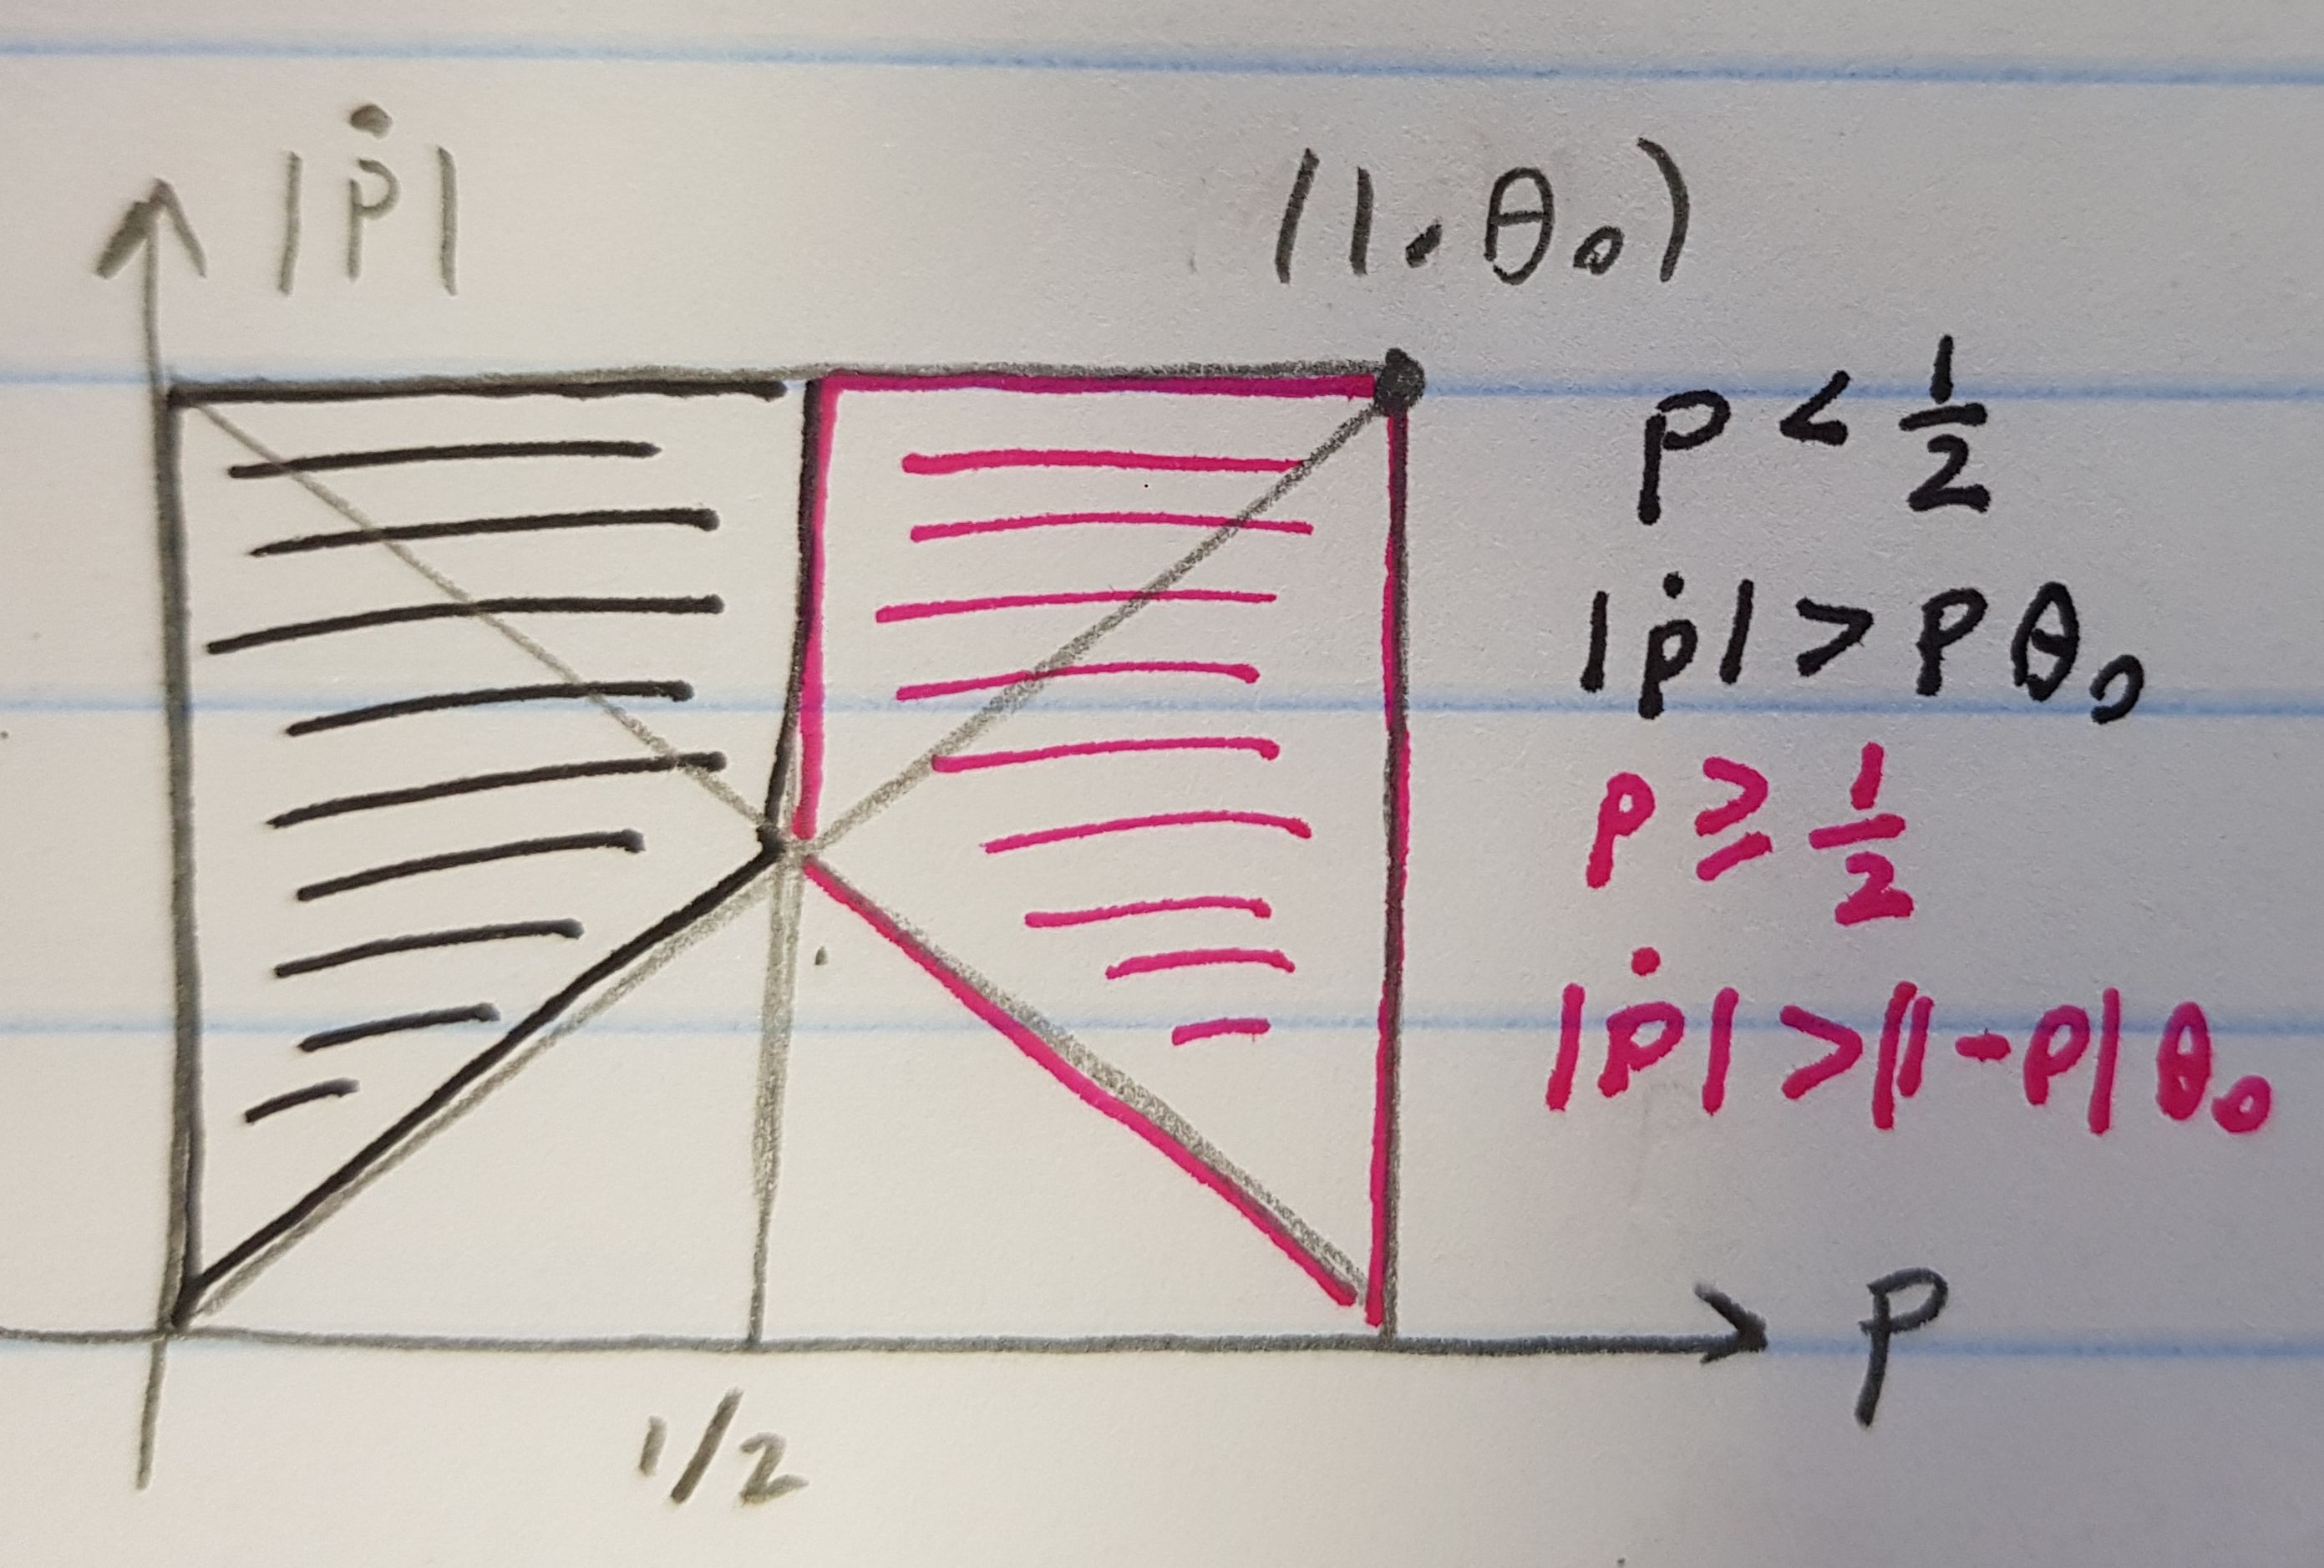
\includegraphics[width=0.9\columnwidth]{20200225_150346.jpg}

\end{columns}

\end{frame}


\setbeamercolor{background canvas}{bg=white!10}
\begin{frame}\frametitle{What about $\dot{\theta}_t$?}

We assume that $p_t$ is near the extremes, and then we do \textbf{not} have $\theta_t=\theta_0$. Also, we assume $\ddot{p}_t\approx0$ (because I do not know how to model it).

\begin{itemize}

\item $p_t<\frac{1}{2}$ and $|\dot{p}_t|>\theta_0p_t$: $\frac{\dot{\theta}_t}{\theta_t}\approx-\frac{|\dot{p}_t|\dot{p}_t}{p_t^2}\frac{p_t}{|\dot{p}_t|}=-\frac{\dot{p}_t}{p_t}$. Then, we have $\lim_{p_t\to0^+}\left[\frac{\dot{\theta}_t}{\theta_t}\right]\approx\lim_{p_t\to0^+}\left[-\frac{\dot{p}_t}{p_t}\right]=-\infty\times\sign(\dot{p}_t)$. In this situation, the drift for $Z_t$ tends to $-\infty\times\sign(\dot{p}_t)$.
\item $p_t\geq\frac{1}{2}$ and $|\dot{p}_t|>\theta_0(1-p_t)$: $\frac{\dot{\theta}_t}{\theta_t}\approx\frac{|\dot{p}_t|\dot{p}_t}{(1-p_t)^2}\frac{(1-p_t)}{|\dot{p}_t|}=\frac{\dot{p}_t}{(1-p_t)}$. Then, we have $\lim_{p_t\to1^-}\left[\frac{\dot{\theta}_t}{\theta_t}\right]\approx\lim_{p_t\to1^-}\left[\frac{\dot{p}_t}{(1-p_t)}\right]=\infty\times\sign(\dot{p}_t)$. In this situation, the drift for $Z_t$ tends to $\infty\times\sign(\dot{p}_t)$.

\end{itemize}
\quad\\
\alert{Maybe we can use a model where $\theta_t=\theta_0$ only in the diffusion. The SDE would remain between 0 and 1, and the Lamperti transform would be simpler.}

\end{frame}


%\setbeamercolor{background canvas}{bg=white!10}
%\begin{frame}\frametitle{Plotting the drift for $Z_t$: ($\theta_t$ and $\dot{\theta}_t$ with artificial definitions)}
%
%\graphicspath{{../../Mathematica_Files/}}
%
%\begin{table}[]
%\begin{tabular}{lll}
% 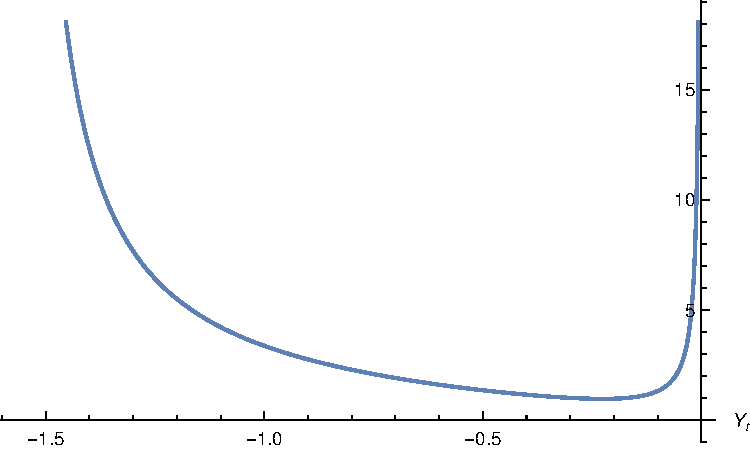
\includegraphics[width=0.3\columnwidth]{drift_z_1.pdf} & 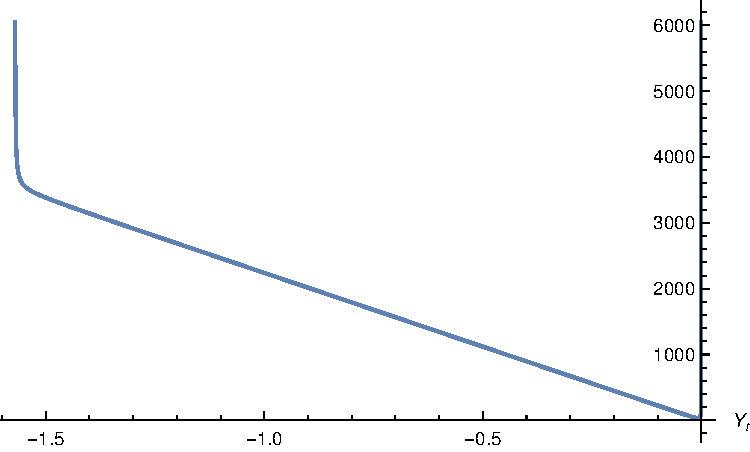
\includegraphics[width=0.3\columnwidth]{drift_z_2.pdf} & 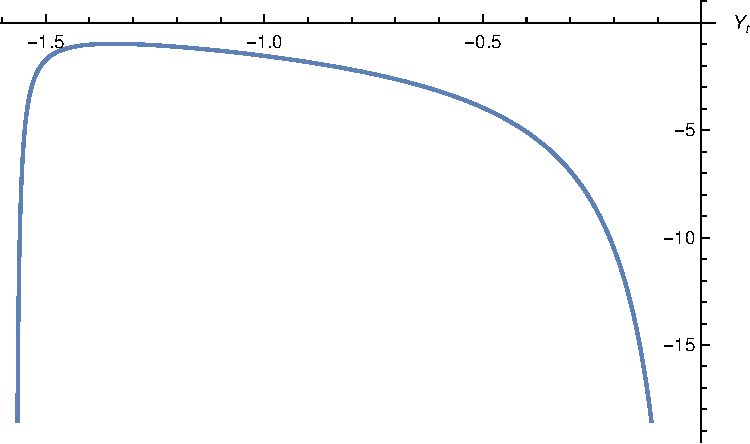
\includegraphics[width=0.3\columnwidth]{drift_z_3.pdf} \\
% {\tiny$p_t=0,\alpha=0.1,\dot{p}_t=1,\theta_t=1,\dot{\theta}_t=0$} & {\tiny$p_t=0,\alpha=0.1,\dot{p}_t=1,\theta_t=1,\dot{\theta}_t=1000$} & {\tiny$p_t=1,\alpha=0.1,\dot{p}_t=-1,\theta_t=1,\dot{\theta}_t=0$} \\
% 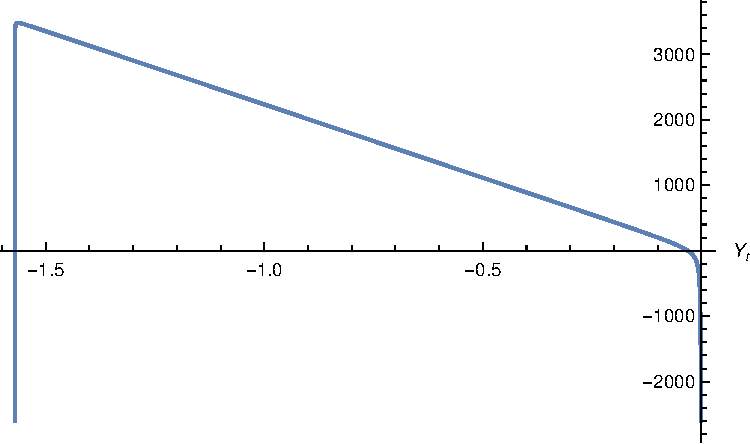
\includegraphics[width=0.3\columnwidth]{drift_z_4.pdf} & 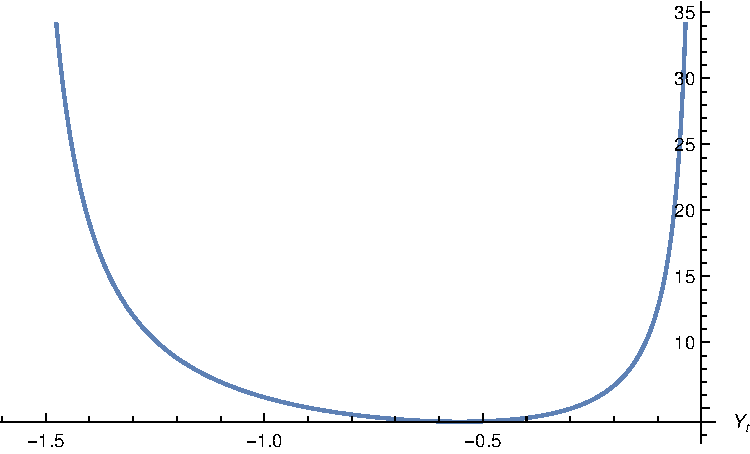
\includegraphics[width=0.3\columnwidth]{drift_z_5.pdf} & 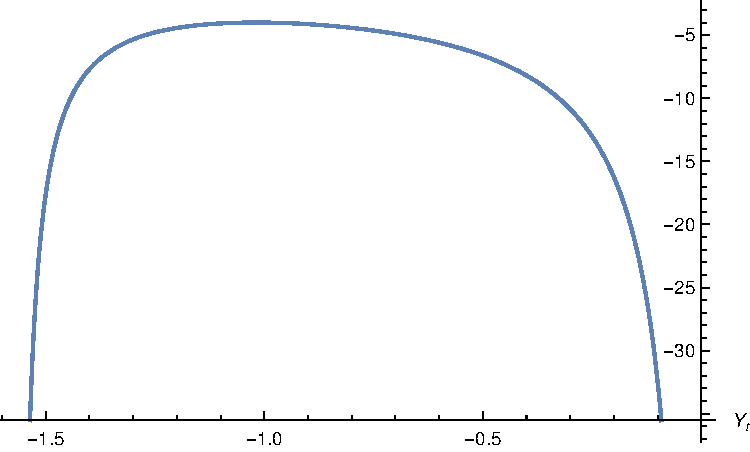
\includegraphics[width=0.3\columnwidth]{drift_z_6.pdf} \\
% {\tiny$p_t=1,\alpha=0.1,\dot{p}_t=-1,\theta_t=1,\dot{\theta}_t=1000$} & {\tiny$p_t=1/2,\alpha=0.1,\dot{p}_t=1,\theta_t=1,\dot{\theta}_t=0$} & {\tiny$p_t=1/2,\alpha=0.1,\dot{p}_t=-1,\theta_t=1,\dot{\theta}_t=0$}
%\end{tabular}
%\end{table}
%
%\end{frame}

\setbeamercolor{background canvas}{bg=white!10}
\begin{frame}\frametitle{$X_t$, $V_t$, $Z_t$, and $Y_t$:}

It is essential to understand what happens with the domain of each process to have a correct intuition about the SDEs.

\begin{enumerate}
\item $X_t\in\alert{[0},{\color{blue}1]}$.
\item $V_t\in\alert{[-p_t},{\color{blue}1-p_t]}$.
\item $Z_t\in\alert{\Big[-\frac{\pi}{\sqrt{2\alpha\theta_t}}},{\color{blue}0\Big]}$.
\item $Y_t\in{\color{red}\Big[-\frac{\pi}{2}},{\color{blue}0\Big]}$.
\end{enumerate}
Notice that none of the changes of variables inverters the domain (red corresponds to red, and blue to blue).

\end{frame}

\setbeamercolor{background canvas}{bg=white!10}
\begin{frame}\frametitle{Plotting the drift for $Z_t$: ($\theta_t$ and $\dot{\theta}_t$ with real definitions, and $\ddot{p}_t=0$)}

\graphicspath{{../../Mathematica_Files/}}

\begin{table}[]
\begin{tabular}{lll}
 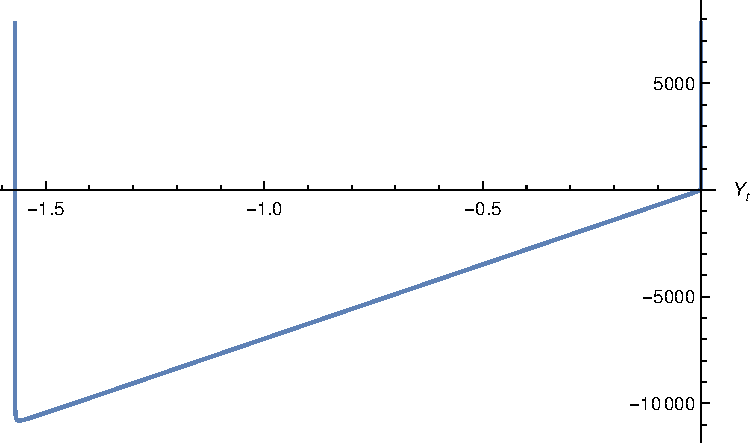
\includegraphics[width=0.3\columnwidth]{drift_z_7.pdf} & 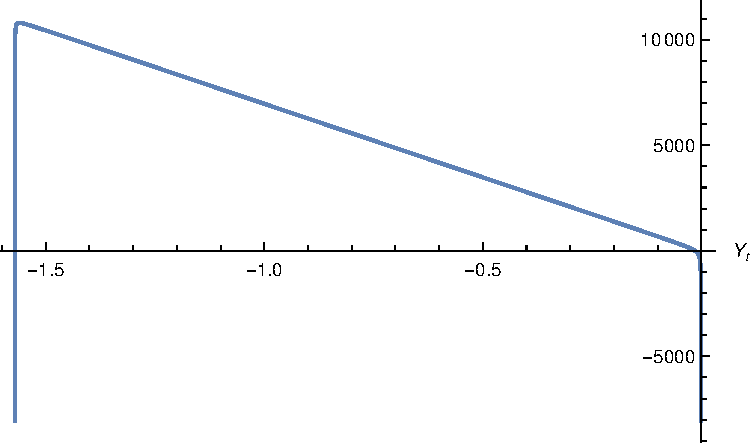
\includegraphics[width=0.3\columnwidth]{drift_z_8.pdf} & 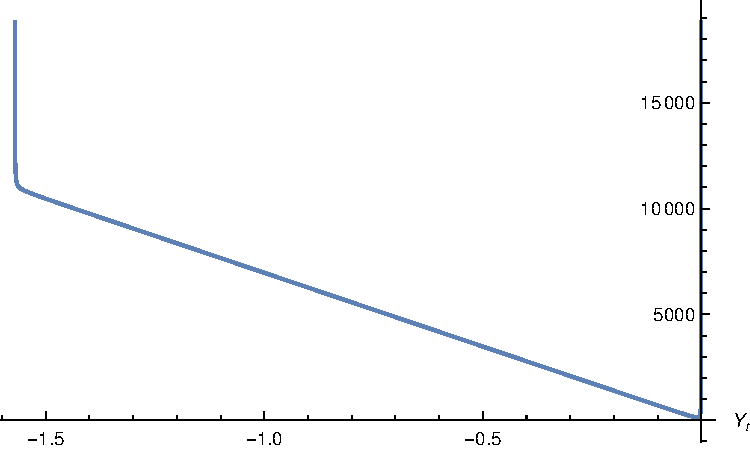
\includegraphics[width=0.3\columnwidth]{drift_z_9.pdf} \\
 {\tiny$p_t=0.01,\alpha=0.1,\dot{p}_t=0.1$ (common case).} & {\tiny$p_t=0.01,\alpha=0.1,\dot{p}_t=-0.1$ (\alert{uncommon case}).} & {\tiny$p_t=0.99,\alpha=0.1,\dot{p}_t=0.1$ (\alert{uncommon case}).} \\
 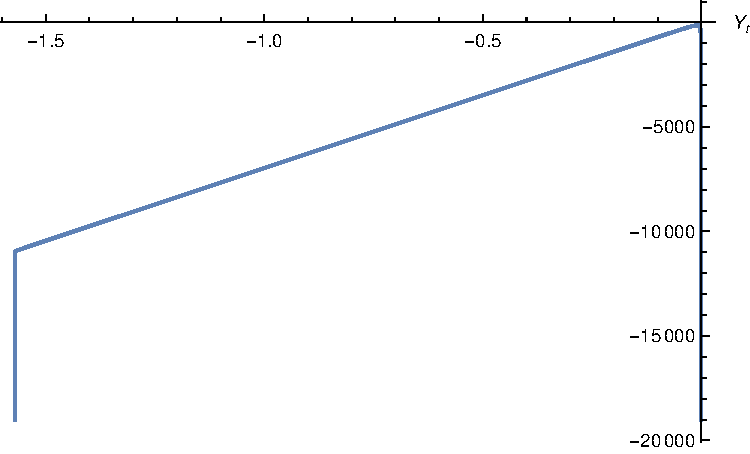
\includegraphics[width=0.3\columnwidth]{drift_z_10.pdf} & 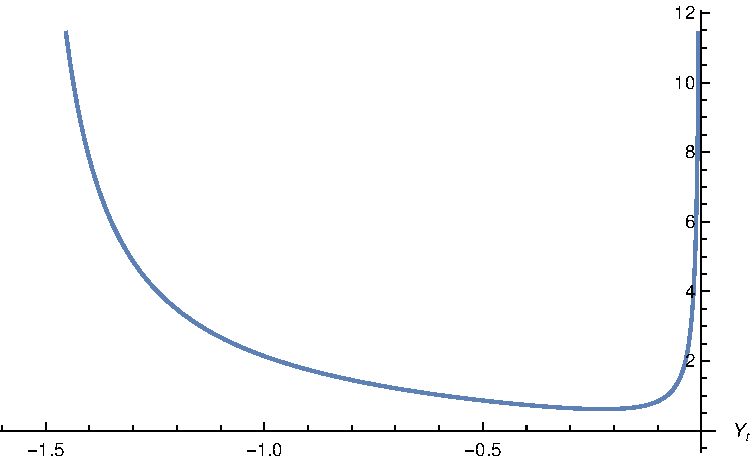
\includegraphics[width=0.3\columnwidth]{drift_z_11.pdf} & 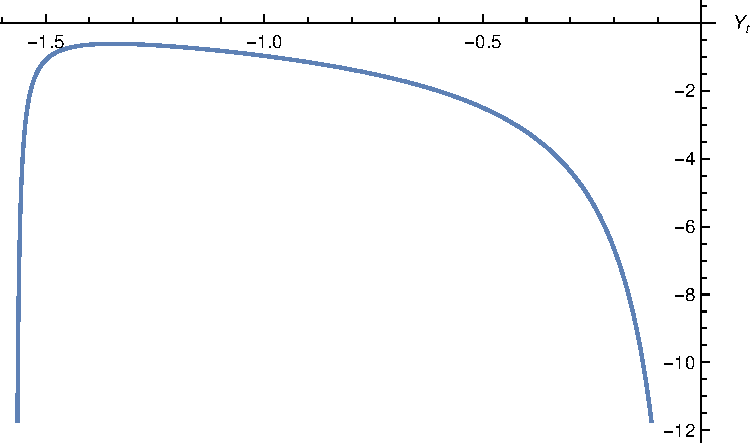
\includegraphics[width=0.3\columnwidth]{drift_z_12.pdf} \\
 {\tiny$p_t=0.99,\alpha=0.1,\dot{p}_t=-0.1$ (common case).} & {\tiny$p_t=1/2,\alpha=0.1,\dot{p}_t=0.2$ (common case).} & {\tiny$p_t=1/2,\alpha=0.1,\dot{p}_t=-0.2$ (common case).}
\end{tabular}
\end{table}

\end{frame}


\setbeamercolor{background canvas}{bg=white!10}
\begin{frame}\frametitle{Plotting the drift for $Z_t$: ($\theta_t$ and $\dot{\theta}_t$ with real definitions, and $\ddot{p}_t=0$)}

\graphicspath{{../../Mathematica_Files/}}

\begin{table}[]
\begin{tabular}{lll}
 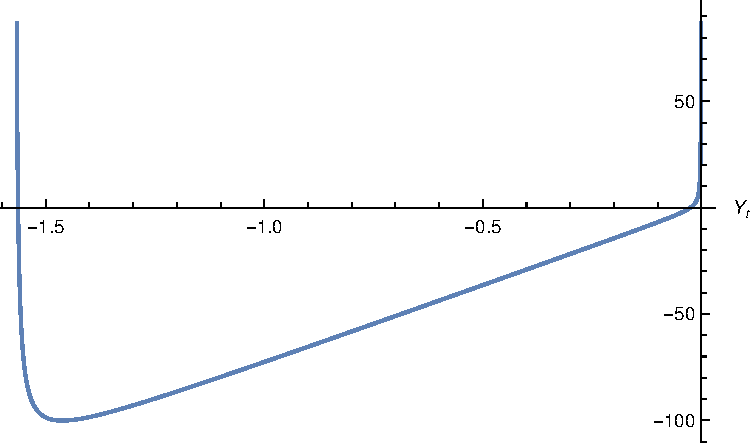
\includegraphics[width=0.3\columnwidth]{drift_z_13.pdf} & 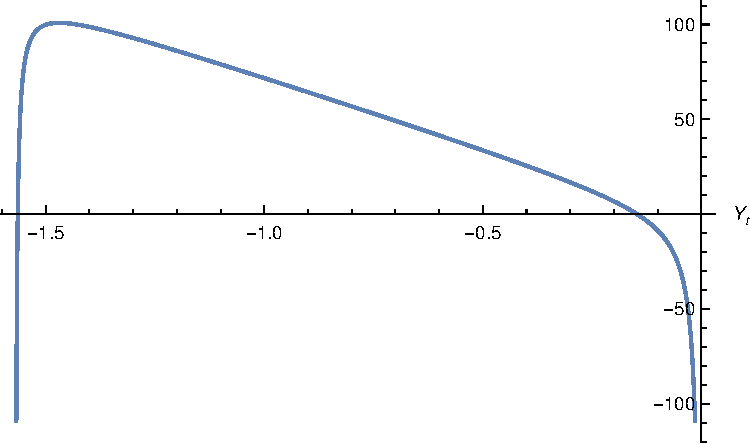
\includegraphics[width=0.3\columnwidth]{drift_z_14.pdf} & 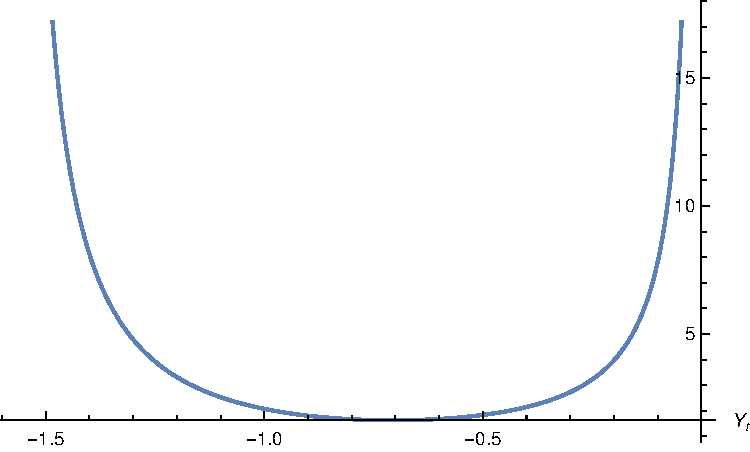
\includegraphics[width=0.3\columnwidth]{drift_z_15.pdf} \\
 {\tiny$p_t=0.1,\alpha=0.1,\dot{p}_t=0.15$ (common case).} & {\tiny$p_t=0.1,\alpha=0.1,\dot{p}_t=-0.15$ (\alert{uncommon case}).} & {\tiny$p_t=0.9,\alpha=0.1,\dot{p}_t=0.15$ (\alert{uncommon case}).} \\
 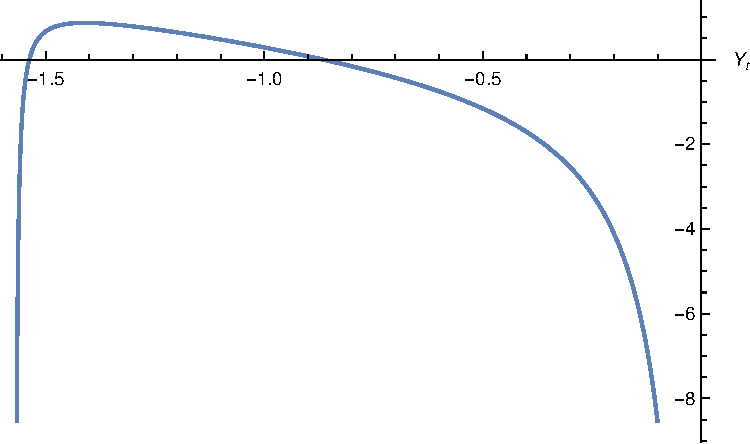
\includegraphics[width=0.3\columnwidth]{drift_z_16.pdf} & 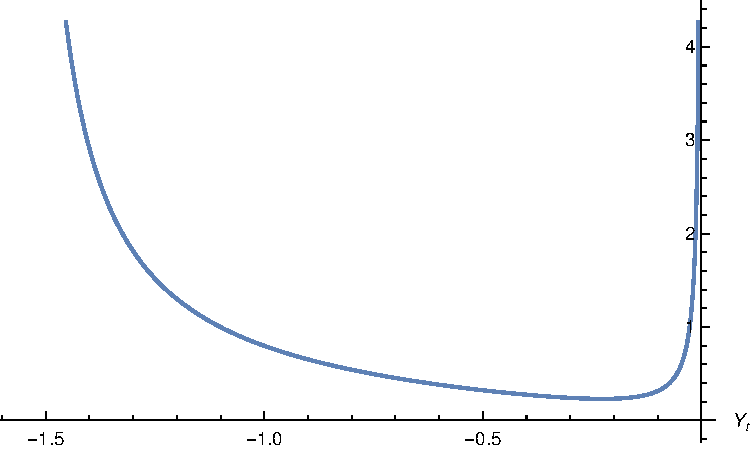
\includegraphics[width=0.3\columnwidth]{drift_z_17.pdf} & 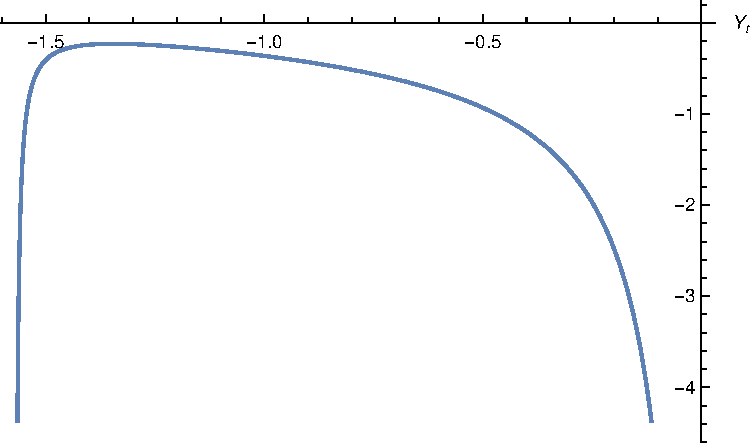
\includegraphics[width=0.3\columnwidth]{drift_z_18.pdf} \\
 {\tiny$p_t=0.9,\alpha=0.1,\dot{p}_t=-0.15$ (common case).} & {\tiny$p_t=0.1,\alpha=0.1,\dot{p}_t=0.05$ (common case).} & {\tiny$p_t=0.9,\alpha=0.1,\dot{p}_t=-0.05$ (common case).}
\end{tabular}
\end{table}

\end{frame}


\setbeamercolor{background canvas}{bg=white!10}
\begin{frame}\frametitle{Professor Kebaier's condition: (In this slide, we remove the time subindex)}

We assume that \textbf{1)} $0<\alpha<\frac{1}{2}$, and \textbf{2)} $\alpha\theta\leq\dot{p}+\theta p\leq(1-\alpha)\theta$.\\
\quad\\
From \textbf{2)}: $\frac{\alpha\theta-\dot{p}}{p}\leq\theta\leq\frac{\theta-\alpha\theta-\dot{p}}{p}$ (recall $p\in[0,1]$, but in this step we assume $p\neq0$). We well check the two inequalities ${\color{red}\frac{\alpha\theta-\dot{p}}{p}\leq\theta}$ and ${\color{blue}\theta\leq\frac{\theta-\alpha\theta-\dot{p}}{p}}$.\\
\quad\\
${\color{blue}\theta(1-p-\alpha)\geq\dot{p}}$ is implied by the more restrictive inequality ${\color{orange}\theta(1-p-\alpha)\geq|\dot{p}|}$. If we assume that $1-p-\alpha>0$ (or equivalently $p<1-\alpha$), we have the more restrictive inequality ${\color{orange}\theta\geq\frac{|\dot{p}|}{(1-p-\alpha)}}$ which implies the {\color{blue}blue one}.\\
\quad\\
\alert{$\theta(\alpha-p)\leq\dot{p}$} is equivalent to ${\color{violet}\theta\geq\frac{\dot{p}}{\alpha-p}}$ assuming that $\alpha-p<0$ (or $p>\alpha$). Now, {\color{violet}violet} is implied by the more restrictive inequality ${\color{brown}\theta\geq\left|\frac{\dot{p}}{\alpha-p}\right|=\frac{|\dot{p}|}{p-\alpha}}$.\\
\quad\\
Combining the two assumptions, we have that \textbf{2)} is true if $\alpha<p<1-\alpha$, and $\theta=\max\left(\theta_0,\frac{|\dot{p}|}{\min(p-\alpha,1-p-\alpha)}\right)$. For very small $\alpha$, we recuperate our classical condition.

\end{frame}


\setbeamercolor{background canvas}{bg=white!10}
\begin{frame}\frametitle{Professor Kebaier's Lamperti SDE:}

If we fix $\theta_t=\theta_0$ in the diffusion in both SDEs (our original one and Kebaier's one), then assuming the new condition $\alpha<p<1-\alpha$, we have that both SDEs share the same Lamperti transform (up to the definition of $\theta_t$ in the drift).

\end{frame}


\setbeamercolor{background canvas}{bg=green!20}
\begin{frame}

{\Huge New Model}

\end{frame}


\setbeamercolor{background canvas}{bg=white!10}
\begin{frame}\frametitle{New model for the SDE: $\theta_t=\theta_0$ in the diffusion}

\begin{enumerate}

\item[$X_t$:] $\dif X_t=\left(\dot p_t-\theta_t(X_t-p_t)\right)\dif t+\sqrt{2\alert{\theta_0}\alpha X_t(1-X_t)}\dif W_t$
\item[$V_t$:] $\dif V_t=-\theta_tV_t\dif t+\sqrt{2\alert{\theta_0}\alpha(V_t+p_t)(1-V_t-p_t)}\dif W_t$

\end{enumerate}
Lamperti transform for $V_t$:
\begin{equation*}
\begin{split}
\psi(V_t,t)=\int\frac{1}{\sqrt{2\alert{\theta_0}\alpha(u+p_t)(1-u-p_t)}}\dif u\Bigg|_{u=V_t}&=-\sqrt{\frac{2}{\alpha\alert{\theta_0}}}\arcsin\left(\sqrt{1-V_t-p_t}\right),\\
&=-\sqrt{\frac{2}{\alpha\alert{\theta_0}}}\arcsin\left(\sqrt{1-X_t}\right).
\end{split}
\end{equation*}

We can see that for every $t=t^*$, the primitive function of $\frac{1}{\sigma(v,t^*)}$ is well defined for all $v\in\left[-p(t^*),1-p(t^*)\right]\subset[-1,1]$ (recall $v=x-p_t$, and $x\in[0,1]$).

\end{frame}


\setbeamercolor{background canvas}{bg=white!10}
\begin{frame}\frametitle{Identities for the Lamperti transform of $V_t$:}

\begin{itemize}
\item $\psi(V_t,t)=-\sqrt{\frac{2}{\alpha\alert{\theta_0}}}\arcsin(\sqrt{1-V_t-p_t})$.
\item $\psi_v(V_t,t)=\frac{1}{\sigma(V_t,t)}$.
\item $\psi_{vv}(V_t,t)=\frac{\dif}{\dif v}\left[\frac{1}{\sigma(V_t,t)}\right]=-\frac{\sigma_v(V_t,t)}{\sigma^2(V_t,t)}=-\frac{1}{\sigma^2(V_t,t)}\cdot\sqrt{\frac{\alpha\alert{\theta_0}}{2}}\frac{1-2V_t-2p_t}{\sqrt{(V_t+p_t)(1-V_t-p_t)}}$.
\item $\psi_t(V_t,t)=\frac{\dot{p}_t}{\sqrt{2\alpha\alert{\theta_0}(V_t+p_t)(1-V_t-p_t)}}$.
\end{itemize}

\end{frame}


\setbeamercolor{background canvas}{bg=white!10}
\begin{frame}\frametitle{SDE for $Z_t=\psi(V_t,t)$: ({\color{green}Verified with Mathematica})}

By It\^o's lemma, if $\psi(v,t)$ is $C^2([-p_t,1-p_t])$ for $v$ and $C^1([0,T])$ for $t$, then:
\begin{equation*}
\dif Z_t=\left({\color{blue}\psi_t}+\psi_v\cdot f+\alert{\frac{1}{2}\psi_{vv}\cdot\sigma^2}\right)\dif t+\psi_v\cdot\sigma\dif W_t.
\end{equation*}
If we substitute the terms related with $\psi(V_t,t)$:
\begin{equation*}
{\footnotesize
\begin{split}
\dif Z_t=&\Bigg[{\color{blue}\frac{\dot{p}_t}{\sqrt{2\alpha\theta_0(V_t+p_t)(1-V_t-p_t)}}}\\
&-\frac{\theta_tV_t}{\sqrt{2\alpha\theta_0(V_t+p_t)(1-V_t-p_t)}}\alert{-\frac{1}{2}\sqrt{\frac{\alpha\theta_0}{2}}\frac{1-2V_t-2p_t}{\sqrt{(V_t+p_t)(1-V_t-p_t)}}}\Bigg]\dif t+1\cdot \dif W_t.
\end{split}}
\end{equation*}
Recall $\alert{Z_t=-\sqrt{\frac{2}{\alpha\theta_t}}\arcsin\left(\sqrt{1-V_t-p_t}\right)}$, where $Z_t\in\Big[-\frac{\pi}{\sqrt{2\alpha\theta_t}},{\color{black}0\Big]}$.
\end{frame}


\setbeamercolor{background canvas}{bg=white!10}
\begin{frame}\frametitle{SDE for $Z_t=\psi(V_t,t)$: ({\color{green}Computed with Mathematica})}

\begin{equation*}
\dif Z_t=\underbrace{\left[\frac{\alpha\theta_0\cos(Z_t\sqrt{2\alpha\theta_0})-\theta_t\cos(Z_t\sqrt{2\alpha\theta_0})+2\theta_tp_t+2\dot{p}_t-\theta_t}{\sqrt{\alpha\theta_0}\sqrt{1-\cos(2Z_t\sqrt{2\alpha\theta_0})}}\right]}_{f(Z_t,t)}\dif t+1\cdot\dif W_t.
\end{equation*}\\
\begin{equation*}
\lim_{z\to0^-}f(z,t)=\infty\times\left[\frac{\sign\left(2\theta_tp_t+2\dot{p}_t+\alpha\theta_0-2\theta_t\right)}{\sign(\alpha)\sign(\theta_0)}\right].
\end{equation*}
\begin{equation*}
\lim_{z\to\left[\frac{-\pi}{\sqrt{2\alpha\theta_0}}\right]^+}f(z,t)=\infty\times\left[\frac{\sign\left(2\theta_tp_t+2\dot{p}_t-\alpha\theta_0\right)}{\sign(\alpha)\sign(\theta_0)}\right].
\end{equation*}
We want to find the correct conditions for $\theta_t$.\\
\quad\\
{\small To simplify the SDE, Mathematica has used: $\sin^2(x)-\sin^4(x)=\sin^2(x)\cos^2(x)=\frac{1}{4}\sin^2(2x)=\frac{1}{8}(1-\cos(4x))$.}

\end{frame}


\setbeamercolor{background canvas}{bg=white!10}
\begin{frame}\frametitle{Limit when $z\to0^-$:}\label{C1}

Recall we have a bijective mapping $Z_t({\color{blue}[0},\alert{1]})={\color{blue}\Big[\frac{-\pi}{\sqrt{2\alpha\theta_0}}},\alert{0\Big]}$.\\
\quad\\
We want $\alpha\theta_0-2\theta_t+2\theta_tp_t+2\dot{p}_t\leq0$ so we do not scape from $x=1$ to $x>1$. Then:
\begin{itemize}

\item If $p_t<1$, we have that ${\color{orange}\theta_t\geq\frac{\alpha\theta_0+2\dot{p}_t}{2(1-p_t)}}$.
\item If $p_t=1$, $\lim_{z\to0^-}f(z,t)=\alpha\theta_0+2\dot{p}_t$.\\
\alert{Then, if $\alpha\theta_0>|2\dot{p}_t|$, we scape from $x=1$ to $x>1$.}

\end{itemize}

\end{frame}


\setbeamercolor{background canvas}{bg=white!10}
\begin{frame}\frametitle{Limit when $z\to\left[\frac{-\pi}{\sqrt{2\alpha\theta_0}}\right]^+$:}\label{C2}

Recall we have a bijective mapping $Z_t({\color{blue}[0},\alert{1]})={\color{blue}\Big[\frac{-\pi}{\sqrt{2\alpha\theta_0}}},\alert{0\Big]}$.\\
\quad\\
We want $2\theta_tp_t+2\dot{p}_t-\alpha\theta_0\geq0$ so we do not scape from $x=0$ to $x<0$. Then:
\begin{itemize}

\item If $p_t>0$, we have that ${\color{orange}\theta_t\geq\frac{\alpha\theta_0-2\dot{p}_t}{2p_t}}$.
\item If $p_t=0$, $\lim_{z\to\left[\frac{-\pi}{\sqrt{2\alpha\theta_0}}\right]^+}f(z,t)=2\dot{p}_t-\alpha\theta_0$.\\
\alert{Then, if $\alpha\theta_0>|2\dot{p}_t|$, we scape from $x=0$ to $x<0$.}

\end{itemize}

\end{frame}


\setbeamercolor{background canvas}{bg=white!10}
\begin{frame}\frametitle{Controlled drift:}

From both {\color{orange}orange} conditions in slides (\ref{C1}) and (\ref{C2}), we create a more restrictive condition:
\begin{equation*}
\max\left({\color{orange}\frac{\alpha\theta_0+2\dot{p}_t}{2(1-p_t)}},{\color{orange}\frac{\alpha\theta_0-2\dot{p}_t}{2p_t}}\right)\leq\frac{\alpha\theta_0+|2\dot{p}_t|}{2\min(1-p_t,p_t)}.
\end{equation*}
Then, we choose
\begin{equation}
\theta_t=\max\left(\theta_0,\frac{\alpha\theta_0+|2\dot{p}_t|}{2\min(1-p_t,p_t)}\right).
\label{NC}
\end{equation}
\alert{Notice that we still need $\alpha\theta_0>|2\dot{p}_t|$ when $\{x=0,p=0\}$ or $\{x=1,p=1\}$.} As we no control over this condition, it is enough to ensure that we never reach these pairs $\{x,p_t\}$.\\
\quad\\
Recall that in the paper, we start by choosing $\theta_t=\max\left(\theta_0,\frac{|\dot{p}_t|}{\min(1-p_t,p_t)}\right)$. Our new condition (\ref{NC}) is mroe restrictive.

\end{frame}


\setbeamercolor{background canvas}{bg=white!10}
\begin{frame}\frametitle{Conditions summary:}

\begin{itemize}

\item Initial condition: $\theta_t^{initial}=\max\left(\theta_0,\frac{|\dot{p}_t|}{\min(1-p_t,p_t)}\right)$
\item New condition from Lamperti: $\theta_t^{lamperti}=\max\left(\theta_0,\frac{\alpha\theta_0+|2\dot{p}_t|}{2\min(1-p_t,p_t)}\right)$. Also, we need that $\alpha\theta_0>|2\dot{p}_t|$ when $\{x=0,p=0\}$ or $\{x=1,p=1\}$. Notice $\theta_t^{initial}\leq\theta_t^{lamperti}$.
\item Professor Kebaier's condition: $0<\alpha<1/2$, $\alpha<p_t<1-\alpha$, and $\theta_t^{kebaier}=\max\left(\theta_0,\frac{|\dot{p}|}{\min(p-\alpha,1-p-\alpha)}\right)$.

\end{itemize}
Now, given $p_t<1/2$, we have that $\theta_t^{lamperti}=\theta_t^{kebaier}$ if $\theta_0=\frac{|2\dot{p}_t|}{p_t-\alpha}$ (assuming that in both cases the maximum is not $\theta_0$). Then, how much each one is restrictive depends on $|\dot{p}_t|$ and $p_t$.\\
Conditions $0<\alpha<1/2$ and $\alpha<p_t<1-\alpha$ implies that we never have $\{x=0,p=0\}$ or $\{x=1,p=1\}$

\end{frame}


\end{document}